% !TEX TS-program = xelatex
% !BIB program = bibtex
% !TeX spellcheck = ru_RU
% !TEX root = talk.tex

\documentclass
  [ russian
  , aspectratio=1610
  ] {beamer}


\input{preamble.tex}
\usepackage{listings}
\makeatletter

\input{pretitle.tex}
\input{title.tex}

\newcommand{\academicGroup}{\my@title@group@ru}
\newcommand{\advisorChair}{\my@title@chair@ru}
\title[Разработка виртуальной машины]{\my@title@title@ru}
\author[\my@title@author@ru]{\my@title@author@ru, группа \academicGroup}
\institute[СПбГУ]{}
\date[]{}
\newcommand{\supervisor}{\my@title@supervisor@ru}
\newcommand{\supervisorPosition}{\my@title@supervisorPosition@ru}
\newcommand{\consultant}{\my@title@consultant@ru}
\newcommand{\consultantPosition}{\my@title@consultantPosition@ru}
\newcommand{\reviewer}{\my@title@reviewer@ru}
\newcommand{\reviewerPosition}{\my@title@reviewerPosition@ru}
\newcommand{\defenseYear}{\my@title@year@ru}

\makeatother
\begin{document}
{
\setbeamertemplate{footline}{}

\begin{frame}
    \vspace{15pt}
    \begin{center}
        \begin{tabular}{c}
            \scriptsize{Санкт-Петербургский государственный университет} \\
            \scriptsize{\advisorChair}
        \end{tabular}
        \titlepage
    \end{center}

    \btVFill

    {\scriptsize
        \textbf{Научный руководитель:}  \supervisorPosition~\supervisor \\
        \textbf{Консультант:}  \consultantPosition~\consultant \\
        \textbf{Рецензент:} \reviewerPosition~\reviewer \\
    }
    \makeatother
    \begin{center}
        \vspace{5pt}
        \scriptsize{Санкт-Петербург\\ \defenseYear}
    \end{center}
\end{frame}
}

\begin{frame}{Введение}
    \begin{itemize}
        \item Язык программирования требует согласованной инфраструктуры: компилятора, промежуточных представлений и среды исполнения
        \item Байткод и виртуальная машина отделяют компиляцию от конкретного
способа запуска программы
      \item  Lama --- учебный язык программирования, разработанный Дмитрием Булычевым для преподавания курса по разработке компиляторов.
      \item Компилятор Lama позволяет компилировать программы только в ассемблер архитектуры
        x86\_64
      \item Виртуальная машина позволит студентам курса использовать Lama на практически любой платформе
      
    \end{itemize}
\end{frame}
\begin{frame}{Обзор инфраструктуры}
    \begin{center}
        \resizebox{0.96\linewidth}{!}{\begin{tikzpicture}[
    x=1cm,
    y=1cm,
    stage/.style={
        draw,
        rounded corners=2pt,
        semithick,
        align=center,
        minimum height=11mm,
        text width=32mm,
        fill=gray!8
    },
    transform/.style={
        draw,
        rounded corners=2pt,
        semithick,
        align=center,
        minimum height=11mm,
        text width=32mm,
        fill=gray!8
    },
    snippetstage/.style={
        draw,
        line width=0.35pt,
        draw=black!30,
        minimum width=37mm,
        minimum height=24mm,
        fill=white
    },
    smstage/.style={
        draw,
        line width=0.35pt,
        draw=black!30,
        minimum width=37mm,
        minimum height=24mm,
        fill=white
    },
    component/.style={
        draw,
        rounded corners=2pt,
        line width=0.35pt,
        draw=black!35,
        align=center,
        minimum height=10mm,
        text width=34mm,
        fill=gray!8
    },
    support/.style={
        draw,
        rounded corners=2pt,
        semithick,
        align=center,
        minimum height=11mm,
        text width=37mm,
        fill=blue!10
    },
    test/.style={
        draw,
        rounded corners=2pt,
        semithick,
        align=center,
        minimum height=11mm,
        text width=37mm,
        fill=green!12
    },
    result/.style={
        draw,
        rounded corners=2pt,
        line width=0.35pt,
        draw=black!35,
        align=center,
        minimum height=10mm,
        text width=34mm,
        fill=orange!14
    },
    note/.style={
        align=center,
        font=\small,
        text width=38mm
    },
    resultlabel/.style={
        align=center,
        font=\small
    },
    flow/.style={->, semithick},
    attach/.style={->, dashed, semithick}
]

\node[snippetstage] (source) at (0,0) {};
\node[transform] (driver) at (4.4,0) {драйвер\\компилятора};
\node[transform, text width=38mm] (language) at (8.6,0) {лексический и\\синтаксический\\анализ};
\node[smstage] (stack) at (13.1,0) {};

\node[anchor=north west, inner sep=0pt] at ($(source.north west)+(0.8mm,-0.8mm)$) {
    \begin{tikzpicture}[x=1mm,y=-1mm]
        \clip (0,0) rectangle (36.4,21.9);
        \node[
            anchor=north west,
            align=left,
            font=\ttfamily\fontsize{4.6}{5.1}\selectfont
        ] at (0.05,0.05)
            {var x, y, z;\\
             \\
             fun zip (x) \{\\
             \ \ case x of Pair (x, y) ->\\
             \ \ \ \ case x of\\
             \ \ \ \ \ \ Nil          ->  Nil\\
             \ \ \ \ | Cons (x, xs) -> case y of\\
             \ \ \ \ \ \ \ \ \ \ \ \ \ \ \ Nil ->  Nil\\
             \ \ \ \ \ \ \ \ \ \ \ \ \ \ | Cons (y, ys) ->\\
             \ \ \ \ \ \ \ \ \ \ \ \ \ \ \ \ Cons (Pair (x, y),\\
             \ \ \ \ \ \ \ \ \ \ \ \ \ \ \ \ \ \ zip (Pair (xs, ys)))\\
             \ \ \ \ \ \ \ \ \ \ \ \ \ \ esac\\
             \ \ \ \ esac};
        \node[anchor=south east, font=\ttfamily\tiny, text=gray!65]
            at (36.8,21.5) {$\ddots$};
    \end{tikzpicture}
};
\node[font=\small, align=center, below=1mm of source] {исходная\\программа};

\node[anchor=north west, inner sep=0pt] at ($(stack.north west)+(0.8mm,-0.8mm)$) {
    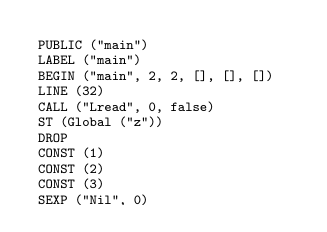
\begin{tikzpicture}[x=1mm,y=-1mm]
        \clip (0,0) rectangle (34.4,22.4);
        \node[
            anchor=north west,
            align=left,
            font=\ttfamily\fontsize{5.0}{5.6}\selectfont
        ] at (0.1,0.25)
            {PUBLIC ("main")\\
             LABEL ("main")\\
             BEGIN ("main", 2, 2, [], [], [])\\
             LINE (32)\\
             CALL ("Lread", 0, false)\\
             ST (Global ("z"))\\
             DROP\\
             CONST (1)\\
             CONST (2)\\
             CONST (3)\\
             SEXP ("Nil", 0)\\
             SEXP ("Cons", 2)};
    \end{tikzpicture}
};

\node[component] (native-backend) at (13.1,2.7) {нативная\\генерация кода};
\node[resultlabel] (native-code) at (17.2,2.7) {нативный код};
\node[support, fill=gray!12, text width=32mm] (execenv) at (15.2,4.4) {среда выполнения};
\node[support, fill=gray!12, text width=32mm] (stdlib) at (19.2,4.4) {стандартная\\библиотека};

\node[resultlabel] (bytecode) at (17.2,0) {байткод};
\node[resultlabel] (stackinterp) at (13.1,-2.8) {интерпретация\\стекового представления};
\node[resultlabel] (sourceinterp) at (8.6,-2.8) {интерпретация\\исходного языка};

% \node[test, text width=34mm] (tests) at (4.4,2.7) {регрессионные\\тесты};

\draw[flow] (source) -- (driver);
\draw[flow] (driver) -- (language);
\draw[flow] (language) -- (stack);

\draw[flow] (stack) -- (native-backend);
\draw[flow] (native-backend) -- (native-code);
\draw[flow] (stack) -- (bytecode);
\draw[flow] (stack) -- (stackinterp);
\draw[flow] (language) -- (sourceinterp);

\draw[attach]   (native-code) -- (execenv);
\draw[attach]  (native-code) -- (stdlib);
% \draw[attach] (tests) -- (driver);

\end{tikzpicture}
}
    \end{center}
    \begin{itemize}
        \item Компилятор поддерживает режим компиляции в байткод, но не существует стандартного
          интерпретатора для него
        \item На данный момент байткод неспецифированный и его запуск многомодульных программ из байткода технически невозможно реализовать
          
    \end{itemize}
\end{frame}

\begin{frame}{Постановка задачи}
  \textbf{Цель:} разработать виртуальную машину байткода языка программирования Lama, согласованную с существующим компилятором в ассемблер x86\_64 \\
    \textbf{Задачи:}
\begin{enumerate}
    \item Реализовать прототип виртуальной машины для существующего формата представления байткода Lama
    \item Доработать формат представления байткода Lama и прототип виртуальной машины для возможности исполнения многомодульных программ

    \item Реализовать виртуальную машину на основе прототипа с предварительным анализом байткода для ускорения выполнения    
    \item Проверить корректность работы виртуальной машины и оценить её производительность на существующих тестах
  \end{enumerate}
\end{frame}


\begin{frame}{Прототип виртуальной машины}
 \textbf{На первом этапе был реализован прототип виртуальной машины\footnote[frame]{\url{https://github.com/ancavar/Lama/
  pull/1}}:}
  \begin{itemize}
    \item Исходный байткод Lama задаёт стековую модель вычислений: инструкции берут аргументы со стека и помещают результат обратно на стек
    \item Значения в среде исполнения представлены в двух формах: fixnum для целых чисел и указатель
      на объект в куче для составных значений
    \item Составные объекты, строки, массивы и замыкания размещаются в куче
    \item Среда исполнения реализована на языке Си, поэтому виртуальная машина использует уже
      существующую инфраструктуру языка
  \end{itemize}

% Там на слайде полезно будет вкратце рассмотреть модель вычислений абстрактной машины: то, что это стековая машина с двумя видами значений (указатель в кучу или fixnum), что у нас есть библиотека времени выполнения на Си, которая предоставляет нам GC и реализации для большинства инструкций
\end{frame}


\begin{frame}{Байткодное представление}
    \centering
    \scriptsize
    \setlength{\tabcolsep}{2pt}
    \renewcommand{\arraystretch}{1.15}
    \begin{tabular}{cccccc}
        \colorbox{green!17}{\strut magic} &
        \colorbox{green!17}{\strut version} &
        \colorbox{gray!12}{\strut string\_table\_size} &
        \colorbox{gray!12}{\strut globals\_count} &
        \colorbox{green!17}{\strut imports\_count} &
        \colorbox{gray!12}{\strut publics\_count}
    \end{tabular}

    \vspace{0.35em}

    \begin{tabular}{cccc}
        \colorbox{gray!12}{\strut string\_table} &
        \colorbox{green!17}{\strut imports} &
        \colorbox{green!17}{\strut publics} &
        \colorbox{gray!12}{\strut code}
    \end{tabular}

    \vspace{0.5em}

    \footnotesize
    Зеленым отмечены поля и секции, добавленные или измененные по сравнению с исходным форматом

    \vspace{0.8em}

    \begin{columns}[t]
        \begin{column}{0.46\linewidth}
            \textbf{Новые записи}
            \begin{itemize}
                \item добавлены магическое число и версия формата байткода
                \item \texttt{imports}: импортированный модули
                \item \texttt{publics}: добавлен флаг для различия публичных функций и глобальных переменных
            \end{itemize}
        \end{column}
        \begin{column}{0.5\linewidth}
            \textbf{Изменения в инструкциях}
            \begin{itemize}
                \item  Добавлено количество замкнутых переменных в качестве операнда
                  \texttt{BEGIN\_CLOSURE}:
                \item Добавлена новая инструкция \texttt{FAIL\_KEEP}
                \item Внешние ссылки кодируются отрицательными операндами через таблицу строк
                \item Вместо инструкций \texttt{read}/\texttt{write}/\texttt{length}/\texttt{string} вызываются непосредственно функции среды исполнения
            \end{itemize}
        \end{column}
    \end{columns}
\end{frame}

\begin{frame}{Архитектура виртуальной машины}
    \begin{center}
        \resizebox{0.96\linewidth}{!}{\begin{tikzpicture}[
    x=1cm,
    y=1cm,
    module/.style={
        draw,
        rounded corners=2pt,
        semithick,
        align=center,
        minimum height=17mm,
        text width=31mm,
        fill=gray!8,
        font=\small
    },
    owner/.style={
        draw,
        rounded corners=2pt,
        semithick,
        align=center,
        minimum height=17mm,
        text width=31mm,
        fill=gray!14,
        font=\small
    },
    boundary/.style={
        draw,
        rounded corners=2pt,
        semithick,
        align=center,
        minimum height=17mm,
        text width=31mm,
        fill=gray!8,
        font=\small
    },
    artifact/.style={
        draw,
        rounded corners=2pt,
        line width=0.35pt,
        draw=black!35,
        align=center,
        minimum height=17mm,
        text width=31mm,
        fill=orange!14,
        font=\small
    },
    flow/.style={->, semithick},
    attach/.style={->, dashed, semithick}
]

\node[boundary] (cli) at (0,0) {\texttt{lama.c}\\консольная\\утилита};
\node[owner] (vm) at (4.4,0) {\texttt{vm.c}};

\node[module] (loader) at (9.3,2.5) {\texttt{loader.c}};
\node[module] (bytecode) at (14.3,2.5) {\texttt{bytecode.c}\\\texttt{bytecode.h}};

\node[module] (converter) at (10.5,0) {\texttt{converter.c}};
\node[module] (ops) at (18.1,0) {\texttt{ops.c}\\обработчики};

\node[module] (symbols) at (10.5,-2.5) {\texttt{symbols.c}\\публичные\\символы};
\node[module] (ffi) at (14.6,-2.5) {\texttt{ffi.c}\\внешние\\вызовы};
\node[boundary] (execenv) at (18.1,-2.5) {среда\\выполнения};

\draw[flow] (cli) -- (vm);
\draw[flow] (vm) -- node[pos=0.58, above left, align=center, fill=white, inner sep=1pt, font=\scriptsize] {загрузка\\юнитов} (loader);
\draw[flow] (loader) -- node[midway, above, align=center, fill=white, inner sep=1pt, font=\scriptsize] {чтение\\байткода} (bytecode);
\draw[flow] (vm) -- node[pos=0.56, above, align=center, fill=white, inner sep=1pt, font=\scriptsize] {декодирование\\и связывание} (converter);
\draw[flow] (converter) --  (ops);
\draw[flow] (converter) -- (symbols);
\draw[flow] (converter) -- (ffi);
\draw[flow] (ops) -- (execenv);
\draw[flow] (vm.south) -- ++(0,-3.35)
    node[pos=0.45, right, align=center, fill=white, inner sep=1pt, font=\scriptsize]
    {подготовка\\сборщика мусора}
    -| (execenv.south);

\end{tikzpicture}
}
    \end{center}
\end{frame}

\begin{frame}{Подготовка кода}
    \begin{center}
        \resizebox{0.92\linewidth}{!}{\begin{tikzpicture}[
    x=1cm,
    y=1cm,
    source/.style={
        draw,
        line width=0.35pt,
        draw=black!30,
        minimum width=37mm,
        minimum height=24mm,
        fill=white
    },
    sourceback/.style={
        draw,
        line width=0.35pt,
        draw=black!25,
        minimum width=37mm,
        minimum height=24mm,
        fill=gray!6
    },
    linkbox/.style={
        draw,
        rounded corners=2pt,
        semithick,
        align=center,
        text width=28mm,
        minimum height=11mm,
        inner sep=3pt,
        fill=gray!10,
        font=\scriptsize
    },
    insn/.style={
        draw,
        semithick,
        align=left,
        text width=16mm,
        minimum height=4.2mm,
        inner sep=1pt,
        fill=orange!18,
        font=\fontsize{5.4}{5.9}\selectfont\ttfamily
    },
    operand/.style={
        draw,
        semithick,
        align=left,
        text width=16mm,
        minimum height=4.2mm,
        inner sep=1pt,
        fill=orange!6,
        font=\fontsize{5.4}{5.9}\selectfont\ttfamily
    },
    operandwide/.style={
        operand
    },
    marker/.style={
        draw,
        semithick,
        align=center,
        text width=16mm,
        minimum height=4.2mm,
        inner sep=1pt,
        fill=gray!8,
        font=\fontsize{5.4}{5.9}\selectfont\ttfamily
    },
    flow/.style={->, semithick}
]

\node[sourceback] at (-4.23,0.44) {};
\node[sourceback] at (-4.34,0.32) {};
\node[source] (bc) at (-4.45,0.2) {};
\node[anchor=north west, inner sep=0pt] at ($(bc.north west)+(0.8mm,-0.8mm)$) {
    \begin{tikzpicture}[x=1mm,y=-1mm]
        \clip (0,0) rectangle (34.4,22.4);
        \node[
            anchor=north west,
            align=left,
            font=\ttfamily\fontsize{5.0}{5.6}\selectfont
        ] at (0.1,0.25)
            {PUBLIC ("main")\\
             LABEL ("main")\\
             BEGIN ("main", 2, 2, [], [], [])\\
             LD (Global ("x"))\\
             CONST (3)\\
             CALL ("func", 0, false)\\
             ST (Global ("z"))\\
             BINOP ("+")\\
             DROP\\
             ...};
    \end{tikzpicture}
};

\coordinate (convStart) at ($(bc.east)+(0.25,0)$);
\coordinate (convEnd) at (-0.20,0.2);
\draw[flow] (convStart) -- (convEnd)
    node[midway, above, font=\small] {конвертер};

\node[linkbox] (links) at (-1.15,-2.35)
    {опережающие ссылки\\
     соответствие индексов};

\node[insn] (c1) at (1.45,1.30) {\texttt{op\_begin}};
\node[operand, anchor=west] (a1b) at (c1.east) {\texttt{2}};
\node[operand, anchor=west] (a1c) at (a1b.east) {\texttt{2}};

\node[insn, below=0pt of c1] (c2) {\texttt{op\_ld\_glo}};
\node[operand, anchor=west] (a2) at (c2.east) {\texttt{\&globals[0]}};

\node[insn, below=0pt of c2] (c3) {\texttt{op\_const}};
\node[operand, anchor=west] (a3) at (c3.east) {\texttt{3}};

\node[insn, below=0pt of c3] (c4) {\texttt{op\_call}};
\node[operand, anchor=west] (a4a) at (c4.east) {\texttt{func}};
\node[operand, anchor=west] (a4b) at (a4a.east) {\texttt{0}};

\node[insn, below=0pt of c4] (c5) {\texttt{op\_st\_glo}};
\node[operand, anchor=west] (a5) at (c5.east) {\texttt{\&globals[2]}};

\node[insn, below=0pt of c5] (c6) {\texttt{op\_add}};

\node[insn, below=0pt of c6] (c7) {\texttt{op\_drop}};

\node[marker, anchor=north west] (dots) at (c7.south west) {\texttt{...}};

\draw[flow] (convEnd) -- (links.north);
\draw[flow] (convEnd) -- (c3.west);

\end{tikzpicture}
}
    \end{center}
    \begin{itemize}
        \item Кодовая секция декодируется в один проход во внутреннее представление для каждого юнита
        \item Проверяются границы инструкций, цели переходов, вызовы и стековая глубина
    \end{itemize}
\end{frame}


\begin{frame}{Тестирование}
      \textbf{Проверка корректности осуществлялась несколькими способами:}
      \begin{itemize}
        \item Регрессионные тесты покрывают известные сценарии исполнения программ Lama
        \item Имеющийся компилятор Lama, запущенный на виртуальной машине, сравнивался с нативным кодом
        \item Фаззинг использовался для поиска ошибок в обработке байткода и исполнения программ
        \end{itemize}
\end{frame}

\begin{frame}{Эксперимент: условия}
    \textbf{Конфигурация тестового оборудования:}
    \begin{itemize}
    \item AMD Ryzen 7 6800H
    \begin{itemize}
      \item каждый запуск привязывался к одному физическому ядру (без одновременной многопоточности)
    \end{itemize}
    \item DDR5 16 ГБ @ 6400 МГц
    \begin{itemize}
      \item без подкачки
    \end{itemize}
    \item Ubuntu 26.04 x86\_64 
    \item gcc Ubuntu 15.2.0-16ubuntu1
    \end{itemize}
\end{frame}

\begin{frame}{Исследовательский вопрос}
    \begin{description}
        \item[RQ:] Какова накладная стоимость виртуальной машины относительно нативного исполнения по времени и памяти на характерных нагрузках Lama?
    \end{description}
\end{frame}

\begin{frame}{Эксперимент: время работы}
    \centering
    \small
    \resizebox{0.98\linewidth}{!}{
    \begin{tabular}{lccccc}
        \toprule
        Набор тестов & нат. & прототип & ВМ & Замедление нат. vs ВМ & $n$ \\
        \midrule
        \texttt{performance/Sort} & 28{,}57 c & 95.5 с & 48{,}85 c & 1{,}71$\times$ & 1 \\
        \texttt{lama\_compiler/regression} & 0{,}1907 c & 0{,}3526 c & 0{,}2526 c & 1{,}33$\times$ & 62 \\
        \texttt{lama\_compiler/regression/expressions} & 0{,}1187 c & 0{,}1926 c & 0{,}1465 c & 1{,}25$\times$ & 998 \\
        \texttt{lama\_compiler/regression/deep-expressions} & 3{,}3754 c & 8{,}5804 c & 4{,}8942 c & 1{,}45$\times$ & 11 \\
        \bottomrule
    \end{tabular}}

    \vspace{0.8em}
    \begin{itemize}
        \item На всех рассмотренных вычислительно содержательных нагрузках \texttt{new-vm} медленнее нативного исполнения
    \end{itemize}
\end{frame}

\begin{frame}{Эксперимент: потребление памяти}
    \centering
    \small
    \resizebox{0.98\linewidth}{!}{
    \begin{tabular}{lccc}
        \toprule
        Тест & нат. & прототип & ВМ \\
        \midrule
        performance/Sort & 200 & 195 & 214 \\
        \texttt{lama\_compiler/regression} & 65144 & 62052 & 63512 \\
        \texttt{lama\_compiler/expressions} & 31412 & 29796 & 29912 \\
        \texttt{lama\_compiler/deep-expressions} & 1038276 & 1091056 & 1124684 \\
        \bottomrule
    \end{tabular}}

    \vspace{0.8em}
    \begin{itemize}
        \item В таблице приведён peak RSS для отдельных характерных тестов в килобайтах.
        \item RSS в пределах погрешности
    \end{itemize}
\end{frame}


\begin{frame}{Заключение}
  В ходе данной работы были решены следующие задачи.
    \begin{enumerate}
        \item Реализован прототип виртуальной машины для существующего формата представления байткода Lama
        \item Доработаны формат представления байткода Lama и прототип виртуальной машины для возможности исполнения многомодульных программ
        \item Реализована виртуальная машина на основе прототипа с предварительным анализом байткода для ускорения выполнения
        \item Проверены корректность работы виртуальной машины и её производительность на существующих тестах
    \end{enumerate}
    Ознакомиться с кодом можно по ссылке \url{https://github.com/ancavar/Lama/new/new-vm/}
\end{frame}


\begin{frame}{Исполнение}
    \begin{center}
        \resizebox{!}{0.62\textheight}{\begin{tikzpicture}[
    x=1cm,
    y=1cm,
    entrycell/.style={
        draw,
        semithick,
        align=left,
        text width=31mm,
        minimum height=5.8mm,
        inner sep=2pt,
        font=\scriptsize
    },
    codecell/.style={
        draw,
        semithick,
        align=left,
        text width=39mm,
        minimum height=5.8mm,
        inner sep=2pt,
        font=\scriptsize
    },
    entryfunc/.style={entrycell, fill=orange!18},
    entryoperand/.style={entrycell, fill=orange!6},
    codefunc/.style={codecell, fill=orange!18},
    codeoperand/.style={codecell, fill=orange!6},
    markerentry/.style={entrycell, fill=gray!8, align=center},
    markercode/.style={codecell, fill=gray!8, align=center},
    handler/.style={
        draw,
        rounded corners=2pt,
        semithick,
        align=left,
        text width=47mm,
        minimum height=8mm,
        inner sep=4pt,
        fill=white,
        font=\scriptsize
    },
    ipbox/.style={
        draw,
        rounded corners=2pt,
        semithick,
        align=center,
        minimum width=8mm,
        minimum height=5mm,
        inner sep=4pt,
        fill=gray!8,
        font=\scriptsize
    },
    flow/.style={->, semithick},
    targetflow/.style={->, semithick, rounded corners=4pt},
    returnflow/.style={->, semithick, densely dashed}
]

\node[font=\small\bfseries, align=center] at (-4.3,0.85) {\\\texttt{entry\_points}};
\node[font=\small\bfseries, align=center] at (0.75,0.85) {\\\texttt{all\_code}};
\node[font=\small\bfseries] at (8.1,0.65) {\texttt{ops.c}};

\node[entryfunc] (entrycall1) at (-4.3,0) {\texttt{func: op\_call}};
\node[entryoperand, below=0pt of entrycall1] (entrytarget1) {\texttt{target: main\_1}};
\node[entryoperand, below=0pt of entrytarget1] (entryargs1) {\texttt{num: 0}};
\node[entryfunc,    below=0pt of entryargs1] (entrydrop1) {\texttt{func: op\_drop}};
\node[markerentry,  below=0pt of entrydrop1] (entrygap) {$\cdots$};
\node[entryfunc,    below=0pt of entrygap]   (entrycalln) {\texttt{func: op\_call}};
\node[entryoperand, below=0pt of entrycalln] (entrytargetn) {\texttt{target: main\_n}};
\node[entryoperand, below=0pt of entrytargetn] (entryargsn) {\texttt{num: 0}};
\node[entryfunc,    below=0pt of entryargsn] (entrydropn) {\texttt{func: op\_drop}};
\node[entryfunc,    below=0pt of entrydropn] (entryeof) {\texttt{func: op\_eof}};


\node[codefunc] (mainbegin) at (0.75,0) {\texttt{func: op\_begin (main\_1)}};
\node[codefunc,    below=0pt of mainbegin]  (constop) {\texttt{func: op\_const}};
\node[codeoperand, below=0pt of constop]    (constarg) {\texttt{num: 42}};
\node[codefunc,    below=0pt of constarg]   (callop) {\texttt{func: op\_call}};
\node[codeoperand, below=0pt of callop]     (calltarget) {\texttt{target: f}};
\node[codeoperand, below=0pt of calltarget] (callargs) {\texttt{num: n}};
\node[codefunc,    below=0pt of callargs]   (aftercall) {следующий обработчик};
\node[markercode,  below=0pt of aftercall]  (gap2) {$\cdots$};
\node[codefunc,    below=0pt of gap2]       (fbegin) {\texttt{func: op\_begin (f)}};
\node[markercode,  below=0pt of fbegin]     (fbody) {$\cdots$ тело функции};
\node[codefunc,    below=0pt of fbody]      (endop) {\texttt{func: op\_end}};

\node[ipbox] (ip) at ($(callop.west)+(-0.9,0)$) {\texttt{ip}};

\node[handler] (hcall) at (8.1,-1.25)
    {\texttt{void op\_call(DECL\_STATE) \{}\\
     \texttt{\hspace*{1.2em}ip++;}\\
     \texttt{\hspace*{1.2em}target = ip->target; ip++;}\\
     \texttt{\hspace*{1.2em}n\_args = ip->num; ip++;}\\
     \texttt{\hspace*{1.2em}PUSH\_FRAME(..., ip,}\\
     \texttt{\hspace*{2.4em}sp + n\_args);}\\
     \texttt{\hspace*{1.2em}ip = target;}\\
     \texttt{\hspace*{1.2em}DISPATCH\_JUMP();}\\
     \texttt{\}}};

\node[font=\large] (handlergap) at (8.1,-3.45) {$\cdots$};

\node[handler] (hconst) at (8.1,-4.35)
    {\texttt{void op\_const(DECL\_STATE) \{...\}}};

\node[handler] (hbegin) at (8.1,-5.50)
    {\texttt{void op\_begin(DECL\_STATE) \{...\}}};

\node[handler] (hend) at (8.1,-6.65)
    {\texttt{void op\_end(DECL\_STATE) \{...\}}};

\draw[flow] (ip.east) -- (callop.west);
\draw[flow] (callop.east) -- (hcall.west);
\draw[flow] (mainbegin.east) -- (hbegin.west);
\draw[flow] (constop.east) -- (hconst.west);
\draw[flow] (endop.east) -- (hend.west);

\draw[targetflow] (entrytarget1.east) -- (mainbegin.west);
\draw[targetflow] (entrygap.east) -- (gap2.west);

\draw[targetflow] (entrytargetn.east) -- (gap2.west);
\draw[targetflow] (calltarget.east) -- ++(0.55,0) |- (fbegin.east);
\draw[returnflow] (hend.west) to[out=180,in=0] (aftercall.east);

\end{tikzpicture}
}
    \end{center}
    \begin{itemize}
        \item Внутреннее представление организовано как шитый код
        \item Стек виртуальной машины выделен отдельно с помощью mmap 
        \item Внешние функции вызываются через интерфейс внешних функций
    \end{itemize}
\end{frame}

\end{document}
